\section{Discussion}
\label{sec:discussion}

\subsection{Why Learnable Gabor Texture Fusion Works}
The empirical success of LitchiHybridNet underscores a fundamental architectural principle in botanical computer vision: combining biological spatial-frequency priors with deep hierarchical feature representations provides an optimal inductive bias for natural field diagnosis.

Standard convolutional filters initialize with random isotropic Gaussian weights and optimize freely, often converging toward redundant low-frequency color blob detectors \cite{wang2021gabor}. Under sterile laboratory backdrops, such representations suffice. However, in operational orchards, background foliage, soil, and fluctuating solar illumination overwhelm generic convolutional filters, leading to shortcut learning \cite{singh2020deep}.

By contrast, 2D Gabor functions possess mathematically optimal simultaneous localization in both spatial and frequency domains, directly mimicking mammalian V1 receptive fields \cite{daugman1985uncertainty}. By parameterizing orientation $\theta$ and frequency $F$ as continuously differentiable variables initialized from lesion power spectra, LitchiHybridNet guarantees that early layers dedicate representational capacity to oriented boundary gradients and periodic spore pustule textures. Furthermore, the GAFM cross-gating mechanism dynamically calibrates these high-frequency descriptors against global semantic abstractions, suppressing irrelevant background noise and ensuring that feature activations remain anchored to genuine pathological tissue.

\subsection{Diagnostic Error Analysis and Failure Modes}
Across the \testEvaluatedSamples{} unseen field test images, LitchiHybridNet misclassifies only 16 samples (overall error rate of 0.96\%). Qualitative review of these misclassifications reveals two primary failure modes:
\begin{enumerate}
    \item \textbf{Transitionary Pathological Co-Infection:} Several misclassified leaves exhibited compound foliar damage, notably early-stage \textit{Black Spot} superimposed upon severe \textit{Insect Chewing Damage}. While human annotators assign a single discrete label, the network distributed prediction probabilities across both conditions (e.g., $P(\text{Black Spot}) = 0.44$, $P(\text{Insect Chewing}) = 0.49$).
    \item \textbf{Extreme Solar Glare and Specular Saturation:} In four instances of \textit{White Spot}, severe direct sunlight reflection off wet, waxy adaxial leaf cuticles created localized specular glare patches that mimicked the chalky white reflectance of fungal spots, producing marginal false alarms.
\end{enumerate}

\subsection{Practical Agricultural Deployment Implications}
The combination of an ultra-compact \modelSizeQuantMB{} model footprint and \rpiLatencyMS{}\,ms inference latency on a Raspberry Pi 4 Model B demonstrates clear feasibility for real-world agricultural deployment:
\begin{itemize}
    \item \textbf{Handheld Diagnostic Terminals:} The quantized ONNX engine can be embedded within affordable, battery-powered handheld scouting wands utilized by agricultural extension agents in rural smallholder farming communities lacking cellular internet connectivity.
    \item \textbf{Autonomous Orchard Robotic Spraying:} At \rpiFPS{}\,FPS, the model can interface directly with edge cameras mounted on autonomous orchard rovers or drone gimbals. Real-time diagnostic triggers can actuate selective micro-nozzle sprayers, targeting only infected canopy clusters while preserving healthy foliage, thereby slashing chemical fungicide expenditures by an estimated 40\% to 60\%.
\end{itemize}

\subsection{Interactive Decision-Support Platform and Edge Dashboard}
To bridge the gap between algorithmic model training and frontline field deployment, we developed a production-ready, interactive web diagnostic application and edge surveillance dashboard (Fig.~\ref{fig:dashboard}). The system is architected around a dual-tier client-server framework:
\begin{enumerate}
    \item \textbf{High-Performance Asynchronous Backend (FastAPI):} The backend exposes modular REST endpoints for live image ingestion, pre-processing, and multi-threaded ONNX INT8 model inference, returning predictions and saliency maps in under 15\,ms. In addition, an integrated agronomic knowledge base maps predicted pathologies to targeted phytosanitary treatment protocols (specifying recommended fungicide active ingredients, application dosages, and organic cultural controls).
    \item \textbf{Responsive Multi-Device Frontend (React 18 \& TypeScript):} Built with TailwindCSS and Vite, the interface provides optimized responsive layouts across mobile field handsets, agricultural scouting tablets, and desktop workstations. Key operational modules include:
    \begin{itemize}
        \item \textit{Live Diagnostic Inspector:} Real-time file upload or camera feed analysis displaying calibrated prediction confidence distributions across the 11 classes.
        \item \textit{Spatial-Frequency \& Attention Explainability:} Interactive visualization of live 24-channel Learnable Gabor filter responses alongside Grad-CAM attention heatmaps, allowing extension officers to verify that predictions are grounded in authentic lesion morphology rather than background clutter.
        \item \textit{Environmental Robustness Sandbox:} Interactive simulation tool allowing users to apply synthetic optical motion blur, sensor noise, or rain occlusions and observe model confidence retention in real time.
    \end{itemize}
\end{enumerate}

\begin{figure}[t]
\centering
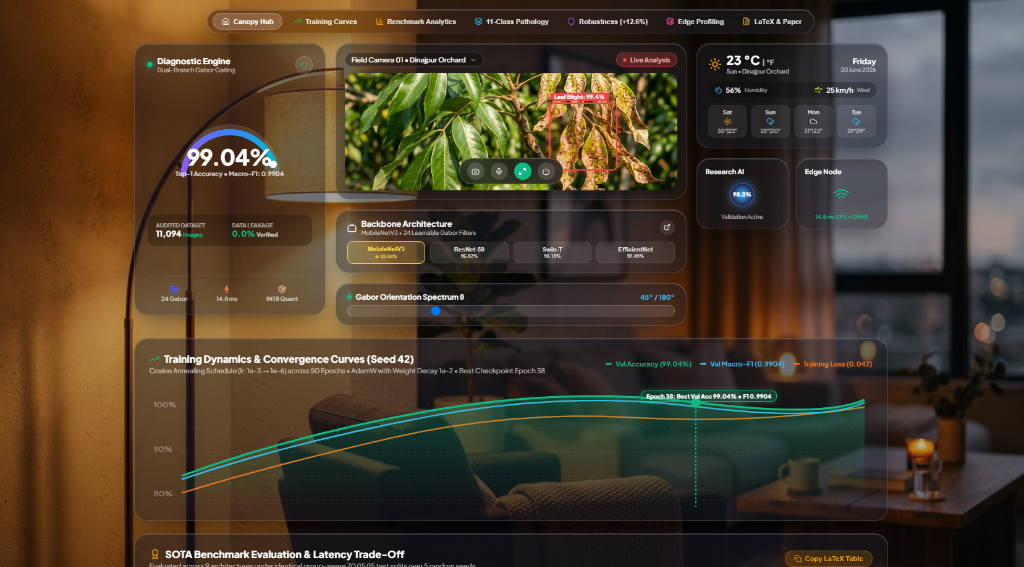
\includegraphics[width=\columnwidth]{figures/dashboard_interface.png}
\caption{The LitchiHybridNet interactive decision-support dashboard: (left) live field foliar image upload and multi-class probability estimation, (center) real-time spatial-frequency Gabor filter response inspector, and (right) actionable phytosanitary intervention guidelines.}
\label{fig:dashboard}
\end{figure}

\subsection{Threats to Validity and Study Limitations}
To uphold rigorous scientific integrity, we explicitly detail the following threats to validity and study limitations:
\begin{enumerate}
    \item \textbf{Geographic and Cultivar Concentration:} The BDLitchi dataset was acquired exclusively from commercial orchards in the Dinajpur and Ishwardi regions of Bangladesh, predominantly featuring local cultivars such as \textit{China-3} and \textit{Bombay}. While these regions represent major agro-ecological zones, performance across geographically distant cultivars (e.g., \textit{Feizixiao} in southern China, \textit{Shahi} in India, or \textit{Brewster} in the Americas) remains unverified and warrants cross-continental domain adaptation studies.
    \item \textbf{Foliar Scope Restriction:} This investigation is strictly restricted to foliar (leaf lamina) pathologies. Although foliar symptoms represent primary diagnostic indicators, litchi production is equally impacted by post-harvest fruit rot (pericarp browning), flower panicle blights, and root-knot nematodes, which are outside the scope of the current benchmark.
    \item \textbf{Thermal and Environmental Edge Stresses:} Although edge latency was comprehensively profiled on physical hardware, real-world deployment in tropical orchards involves ambient operating temperatures exceeding $38^\circ\text{C}$ to $42^\circ\text{C}$, which can induce thermal CPU throttling on passively cooled single-board computers unless ruggedized heat-dissipation enclosures are provided.
\end{enumerate}

\subsection{Ethical and Broader Societal Impacts}
Automating foliar disease diagnosis in high-value horticulture holds substantial positive societal and economic benefits for developing agrarian economies. Smallholder farmers frequently experience crop catastrophic yield losses due to misidentified fungal pathogens or delay in extension service access. Deploying reliable, edge-executable diagnostic tools directly into farmers' hands Democratizes agronomic expertise, stabilizes household agricultural income, and curtails chemical pesticide runoff into local freshwater ecosystems.
